\subsection{DNS – het internet zijn directory dienst}

Een gedistribueerde database die is geïmplementeerd in een hiërarchie van DNS-servers.\\\\
Een applicatielaag-protocol waarmee hosts en DNS’s kunnen communiceren om de domeinnaam achter een IP-adres te vinden.

\subsubsection{Diensten voorzien door DNS}

$\Rightarrow$ Hostname naar IP-adres vertalen.


\begin{itemize}
  \item \textbf{Host aliasing}. Een gecompliceerde host naam kan meerdere aliassen hebben. Een DNS kan opgeroepen worden door een applicatie om het canonical hostname te halen voor een gegeven alias.
\item \textbf{Mail server aliasing}. Het is zeer wenselijk dat email adressen mnemonisch zijn. Het MX record laat toe dat een bedrijf zijn mail en web server dezelfde alias hebben.
\item \textbf{Loadbalancing / Load distribution}. Wordt ook gebruikt om de load distribution over gerepliceerde server te doen. Voor een gerepicleerde web server, is er een verzameling van IP adressen die geassocieerd zijn met één canonical hostname. Wanneer een client een DNS aanvraag doet voor zo’n web server, wisselt de DNS server telkens de volgorde van de IP adressen.
\end{itemize}

\noindent \textit{\textbf{Gang van zaken:}}\\

\noindent Het IP-adres opzoeken achter een webadres (bv. www.google.com)

\be
\itf De host voert de cliëntcomponent van de DNS-applicatie uit
\itf De browser filtert de hostnaam (www.google.com) uit de URL en verzendt de hostnaam naar de clientcomponent van de DNS-applicatie
\itf De DNS-client verzendt een verzoek, dat de hostnaam bevat, naar een DNS-server
\itf De DNS-client krijgt op een gegeven moment antwoord van de DNS-server (het IP)
\itf Dit IP wordt dan gebruikt door de browser om een TCP verbinding te maken met dat IP-adres.
\ee

\clearpage

\subsubsection{Overzicht hoe DNS werkt}

Een applicatie roept de DNS op, met een hostname die vertaald moet worden. De DNS in de gebruiker zijn host neemt dan over, zend een query bericht in het netwerk. Alle DNS query en antwoord berichten zijn verzonden met UDP datagrammen. Na een vertraging, krijgt de DNS in gebruikers host een DNS antwoord die de gewenste mapping voorziet. Deze mapping wordt dan verder doorgegeven naar de applicatie.
Vanuit het standpunt van de applicatie, is DNS een zwarte doos die een simpele eenvoudige vertaal dienst levert. Maar dit is in feite zeer complex. Het bestaat uit meerdere DNS servers die verspreid zijn over de wereld.
Een simpel ontwerp voor DNS zou één DNS server zijn die alle mappings bevat. In dit gecentraliseerd ontwerp, bevelen de clienten hun queries naar deze enkele DNS server, en de DNS server antwoord onmiddellijk terug. Hoewel de gemakkelijkheid van dit ontwerp aantrekkelijk lijkt, is het niet gepast voor deze grote en groeiende aantal hosts. \textbf{De problemen hierbij zijn:}

\begin{itemize}
    \item \textbf{Single point of failure}. Als de DNS crashed, dan ook het internet
\item \textbf{Traffic volume}. De enkele DNS zal alle DNS queries moeten behandelen.
\item \textbf{Distant centralized database}. Een enkele DNS server kan niet dicht bij alle querying clienten liggen. Mensen van de andere kant van de wereld kunnen over trage verbinden gaan, dus dit zal dan leiden tot grote vertragingen.
\item \textbf{Maintenance}. Een enkele DNS server zal alle internet hosts moeten bijhouden. Dit zal niet enkel een grote database opleveren, maar het moet ook regelmatig ge-update moeten worden voor elke nieuwe host.
\end{itemize}

\begin{figure}[h]
\centering
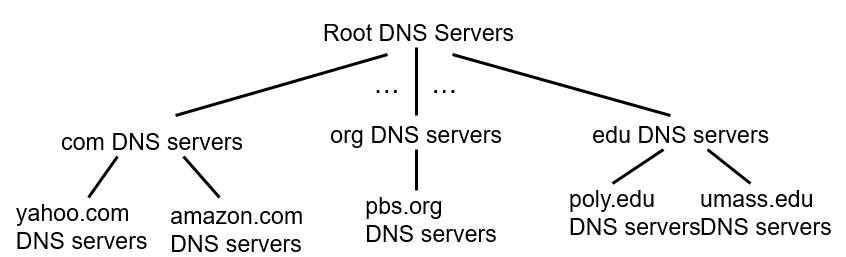
\includegraphics[width=6in]{./img/imghfdst2/hdst2puntje10.png}
\caption{Voorbeeld van een dns hierarchie }
\label{fig:dns hierarchie}
\end{figure}


\clearpage

\subsubsubsection{Een verdeelde hiërarchische databank}

Om om te gaan met het probleem van de schaal, gebruikt DNS een groot aantal servers die in een hiërarchische manier georganiseerd en verdeeld zijn over de wereld. Geen enkele DNS server heeft alle mappings van alle hosts. In plaats daarvan zijn ze verdeeld over alle DNS servers. Er zijn drie klassen van DNS server (Root, top-level domain en authorative).

\begin{itemize}
    \item Root DNS servers. Er zijn 13 root DNS servers. Elke server is eigenlijk een netwerk van gerepliceerde servers, voor zowel beveiligings als vertrouwelijke doeleinden.
    \bi
    \itf contacts authoritative name server if name mapping not known
    \itf gets mapping
    \itf returns mapping to local name server
    \ei
\item Top-Level domain (TLD) servers. Deze servers zijn verantwoordelijk voor top level domeinen zoals com, org, net en alle landelijke domeinen.
\item Authorative DNS servers. Elke organisatie met publieke toegankelijke hosts op het internet moeten publiek toegankelijke DNS records voorzien die de namen van deze hosts naar IP adressen mapped. Een organisatie zijn authorative DNS server bewaart deze DNS records. Een organisatie kan kiezen om zijn eigen authorative DNS server te implementeren om deze records bij te houden. Een alternatief is dat de organisatie kan betalen om deze records op te laten slaan in zo’n server van een service provider.
\end{itemize}

Er is nog een belangrijk type van DNS server die de local DNS server wordt genoemd. Een locale DNS behoort niet strict tot de hierarchie van servers, maar is niet te min centraal aan het DNS architectuur. 

\subsubsubsection{DNS caching}

\textbf{DNS-caching}: Een DNS-server kan wanneer deze een DNS-antwoord ontvangt, de verwijzing in het lokale cachegeheugen plaatsen. (Wordt vooral gebruikt bij recursieve verzoeken)\\

\noindent DNS caching is een zeer belangrijke kenmerk van het DNS systeem. DNS gebruikt dit zeer hard om de vertaging prestatie te verbeteren en de aantal DNS berichten die rond gaan te verminderen. In een query ketting, wanneer een DNS server een DNS antwoord ontvangt, kan het deze mapping in zijn locaal geheugen cachen. Als een hostname/IP adres paar gemapped zijn en er een andere query komt voor dezelfde hostname, kan de DNS server de gewenste IP adres voorzien, zelf als niet authoritative is voor de hostname. Omdat hosts en mappings tussen hostnames en IP adressen geenszins permanent zijn. Daarom doen DNS servers hun gecached om de zoveel tijd weg.

\clearpage

\subsubsection{DNS records en berichten}

\textbf{Bronrecords}: records waarin de hostnaam met bijbehorend IP staat opgeslagen (samen met TTL en Type)\\
Formaat bronrecord: (name, value, type, ttl)

De DNS servers die samen de DNS gedeelde databank implementeren bewaren resource records (RRs). Elke DNS reply bericht draagt één of meerdere RR mee. Een RR bevat de volgende velden:
(Name, Value, Type, TTL)

De betekenis van Name en Value hangen af van Type:
\begin{itemize}
   \item Type = A : dan is Name de hostname en Value het IP adres voor de hostname.
 \item Type = NS : dan is Name het domein en Value is de hostname van een authoritative DNS server die weet hoe het IP adres voor host in het domain op te halen.
 \item Type = CNAME : dan is Value een canonical hostname voor de alias hostname Name.
 \item Type = MX : dan is de Value het canonical name van de mail server die een alias hostname Name.
\end{itemize}


\subsubsubsection{DNS Berichten}

DNS heeft enkel twee mogelijk berichten (Query en reply). Beide berichten hebben dezelfde opmaak. De verschillende velden in een DNS bericht zijn als volgt:
\begin{itemize}
   \item De eerste 12 bytes is de header sectie. Heet eerste veld identificeerd de query. Deze identificator wordt gekopieerd naar het reply bericht. Er zijn een aantal vlaggen in het vlag veld. Deze duiden aan of het een Query of reply bericht is, of de DNS server een authoritatieve server is. En een recursie vlag wanneer de client verlangt dat de DNS een recursieve zoek actie onderneemt als het de record niet heeft.
\item Het \textbf{vragenveld} bevat info over het verzonden verzoek. Deze sectie bevat een naam veld, een type veld.
\item Het \textbf{antwoordenveld} bevat de bronrecords voor de DNS waarvoor het oorspronkelijke verzoek werd verzonden
\item Het autorisatieveld bevat gegevens van andere autoritaire DNS’s
\item DHet aanvullingsveld bevat de aanvullende bronrecords
\end{itemize}


\subsubsubsection{Records toevoegen aan de DNS database}

\textbf{Registrar}: commerciële entiteit die controleert of een domeinnaam uniek is, de domeinnaam in de DNS plaatst en daar geld voor vraagt.

\clearpage

\subsubsection{DNS aanvallen}

\subsubsubsection{DDoS attacks}

\bi
\itf Bombard root servers with traffic
    \bi
    \itf Not successful to date
    \itf Traffic Filtering
    \itf Local DNS servers cache IPs of TLD servers, allowing root server bypass
    \ei
\itf Bombard TLD servers
    \bi
\itf Potentially more dangerous
    \ei
\ei

\subsubsubsection{Redirect attacks}

\bi
\itf Man-in-middle
    \bi
    \itf Intercept queries
    \ei
\itf DNS poisoning
    \bi
    \itf Send bogus relies to DNS server, which caches
    \ei
\ei

\subsubsubsection{Exploit DNS for DDoS}

\bi
\itf Send queries with spoofed source address: target IP
\itf Requires amplification
\ei

\subsection{Peer-to-peerapplicaties}

\subsubsection{P2P-bestandsdistributie}

\textbf{Torrent}: de verzameling peers die deelnemen aan de distributie van een bepaald bestand. Wanneer een peer deelneemt aan een torrent, downloadt hij het bestand in zogenaamde \textbf{chunks} dit zijn kleine deeltjes van het bestand. Wanneer een peer alle chunks heeft verzameld, heeft hij het gehele bestand tot zijn beschikking. De peer uploadt ook zijn chunks wanneer hij ze aan het downloaden is.\\\\
\textbf{Tracker}: Infrastructuurnode van een torrent. Wanneer een peer aan een torrent gaat deelnemen, meldt hij dit aan de tracker. Wanneer een peer zich aanmeldt, selecteert de tracker een willekeurig aantal peers waarmee de peer dan een TCP-verbinding moet leggen om zo onderling chunks te kunnen uitwisselen.\\\\
\textbf{Rarest-first}: Het principe dat gebruikt wordt wanneer een peer een chunk moet gaan halen bij andere peers. Het houdt in dat de peer de chunk die het minst voorkomt in de lijst met chunks die beschikbaar zijn bij de peers, eerst gaat downloaden.

\subsubsection{Gedistribueerde hashtabellen}

\textbf{Overlaynetwerk}: virtueel netwerk dat gemaakt wordt bovenop het bestaande netwerk tussen de peers.